\chapter{Present and future ground-based detectors}

\author[Giacomo Ciani and Paul Fulda]{G.Ciani and P.Fulda\footnote{To be published in \textit{An overview of Gravitational Wave Theory and Detection.}, eds. G. Auger and E. Plagnol (World Scientific, 2016).}}
\address{University of Florida, Gainesville, FL 32611, USA}


\bigtoc

\tableofcontents

\body


\newpage
\begin{abstract}
	\textit{\textbf{Abstract}:
%		the direct detection of gravitational waves by the Advanced LIGO project on the centenary of their prediction by Einstein was a milestone event  for general relativity, gravitational physics, astrophysics and many other related fields.
%		Given the astonishingly small amplitude of the gravitational waves emitted by even the strongest sources, building an instrument sensitive enough to detect these tiny ripples in space-time was deemed impossible by Einstein himself.
%		Only the bright ideas of visionary physicists and many decades of intense scientific research and technological development have made the feat possible.
		In this chapter, we first briefly review the early history of gravitational wave detection, and how the research turned towards the large scale interferometers that proved to be the most effective devices for gravitational wave astronomy.
		We provide an overview of what is generically defined the ``first generation'' of interferometric detectors, a number of instruments built around the globe at the end of the last century, and differing in size, technology and scope.
		A more detailed description is dedicated to the ``second generation'', or ``advanced detectors'', and their main subsystems, which represent the state of the art of the science and technology in the filed.
		In the final section, we give a glimpse of what the next generation of detectors may look like.
		Given the many similitudes between different projects, throughout the chapter we will use LIGO as the leading example, and highlight how the other projects compared to it both technologically and strategically. This choice is mainly due to the size of the LIGO project and of the LIGO Scientific Collaboration, and to the pivotal role they played in the history of the field and eventually in the first detection of gravitational waves. It is important to note, however, that the comparatively small amount of space and detail dedicated to other endeavors is not indicative of the importance of the role they have played and still play in the field.
		}
\end{abstract}


\body


\newpage
\subsection{The first generation of interferometric detectors}\label{subsec:history}

In 1994, NSF approved funding for the construction of the two experimental facilities of the LIGO (Laser Interferometric Gravitational-wave Observatory) project, despite skepticism and some strong opposition from part of the physics and astronomy communities: many thought that the investment, the largest ever made by NSF on a single project, was too risky, that it would needlessly drain resources from other research, and that the chances of success would be almost non existent. History will prove them wrong.
Ground was broken the same year in Hanford, WA, and the following one in Livingston, LA; the construction of the buildings and of the vacuum system, by some measures the biggest ever built at the time, took almost five years. Separated by almost 3000 km, the two experimental sites shared the same basic design, and 4-km long L shape structure; they however differed for the orientation, and for the fact that the one in Hanford was design to accommodate two parallel interferometers in the same vacuum system. The installation of the scientific equipment started in 1999 and was completed by 2002. In the meanwhile, a broader scientific community had grown around the LIGO project, and had taken the shape of two institutions: the LIGO laboratory, in charge of managing the facility and most of the research and development directly aimed at improving the instruments, and the LIGO Scientific Collaboration (LSC), formed by research groups around the world involved in technical and scientific research related to LIGO.
While construction of the two LIGO detectors was ongoing in the US, parallel efforts were being pursued in Europe. A French-Italian collaboration secured funding for a similar facility to be built in Cascina, near Pisa, in Italy. The construction of the 3-km long VIRGO interferometer started in 1996 and was completed in 2003. During this period, the European Gravitational Observatory (EGO) consortium was created to operate the detector and promote gravitational research in Europe. United Kingdom and Germany also joined forces to build the a large scale interferometer; the full-size project was not funded, but was de-scoped to a slightly smaller version named GEO600 (due to its 600 meters long arms), whose construction near Hannover, Germany, started in 1995.
Smaller scale interferometers, mainly intended as prototypes, were build or proposed in other parts of the world. In particular, ACIGO in Australia and CLIO and TAMA300 in Japan.
Among the major players, the first large-scale interferometers to start science observations were the LIGO detectors in 2002, alternating 

%TODO: things that can (must) be added, in loose order of importance
% names of major personalities
% name of institutions
% references
% detail of single and joint science runs of major detectors
% collaboration between LSC and VIRGO
 

\section{Design and operation of the first generation of interferometric gravitational wave detectors}\label{subsec:1stgen}

Despite the extensive research and development effort put forward and the experience acquired over several years on smaller prototypes, it was clear to the gravitational wave community and to the funding agencies that building and operation of km-scale interferometers at their design sensitivity was a high risk, although potentially high gain, endeavor.
The first generation
\footnote{In this and the following sections we describe the initial generation of ground based gravitational wave detectors and their subsequent major upgrades, often referred to as second generation. While this classification matches closely the upgrade history of the two largest scale interferometers, LIGO and Virgo, this may not necessarily be the case for other detectors that adopted different upgrade strategies or started development later. For these interferometers, the distinction that we make here between first and second, or even future, generations is to some degree arbitrary.
} 
of interferometers were designed to be relatively simple, reducing the odds of an actual detection but increasing the chances of their successful commissioning and operation.
In particular, while the adopted topology was very similar to the one used in the subsequent generation, the complexity of many subsystems were kept to a minimum.
The detector infrastructures constituted the bulk of the initial budgets however, and were built to be able to support future upgraded detectors.

\subsection{Initial and Enhanced LIGO}
The initial LIGO detectors\cite{Abbott_2004,Abbott_2009} were power-recycled, Fabry-Perot Michelson interferometers, as schematically represented in the left diagram of \autoref{fig:detector_layouts}.
An out-of-vacuum, 10\,W, 1064\,nm Nd:YAG pre-stabilized laser was phase modulated to add three sets of sidebands for alignment and sensing control.
The beam was then spatially filtered and further stabilized in power and frequency by an in-vacuum input-optics section: this included a 24\,m round-trip suspended triangular optical cavity, referred to as input mode cleaner, a Faraday isolator, and a suspended telescope to match the beam mode to that of the rest of the interferometer.
The beam was then injected into the recycling cavity, which increased the input power seen by the rest of the interferometer by a factor of about 50; finally, the power reached about 20 kW in the arm cavities, designed to have a finesse of 220. There was no signal recycling cavity, and the strain signal was obtained using RF readout of the interferometer output.

The vacuum system layout, also designed to accommodate subsequent upgrades of the detectors, was based on a series of vacuum chambers of either of two types: horizontal ones, for the input and output optics, and vertical ones for the core optics.
Both type are cylinders about 2\,m in diameter and 3\,m in height, with large access ports for easy installation of heavy equipment.
The corner station at the Livingston observatory hosts 6 horizontal chambers, 3 on the input and 3  on the output branch, and 3 vertical chambers, with another two hosted in the end stations.
All chambers, including the ones at the end stations, are connected by 1.2\,m diameter vacuum tubes.
At Hanford, the need to accommodate a second interferometer required doubling the number of chambers, although most of the vacuum tubes were shared by the two laser beams and only minimal additions were needed to connect the extra chambers.

Each chamber was equipped with an optical table, passively isolated from seismic vibrations by a 4-stage spring-mass system, providing about 6 orders of magnitude isolation at 100\,Hz\cite{Giaime_1996}.
Single pendulum suspensions were used to support the most critical optical components, and in particular the 10\,kg, 25\,cm diameter end mirrors of the Fabry-Perot arm cavities, referred to as the input and output test masses; for these optics, the pendulum suspensions provided further 4 orders of magnitude suppression of ground motion at 100\,Hz.
In Livingston, where the ground motion is significantly higher than in Hanford, an out-of-vacuum hydraulic pre-isolation system was added to contribute another factor 10 suppression between 0.1 and 10\,Hz.

Before being decommissioned in 2010 to allow for the installation of the Advanced LIGO hardware, the LIGO detectors were fitted with a number of incremental upgrades\cite{Aasi_2015} meant to improve the sensitivity and allow for prototyping some of the technologies needed for the next generation of instruments.
The laser power was increased for 10\,W to 35\,W;
the thermal compensation system, which had been added to the initial detectors to correct for thermal lensing effects, was further improved to better handle the higher circulating power;
finally, a \textit{DC readout} detection scheme was implemented, in which the interferometer was operated with a slight offset from the dark fringe and the gravitational wave signal was read directly as a modulation of the power on the photodiode.
This required the installation of an output mode cleaner to filter out the RF control sidebands and higher-order spatial modes of the carrier light.
This version of the detectors is referred to as Enhanced LIGO (eLIGO), and conducted science operations in 2009 and 2010. 

\subsection{Virgo and Virgo+}\label{sec:Virgo}
The Virgo detector\cite{Accadia_2012}, in Italy, was based on a design similar to that of LIGO, except with 3\,km Fabry-Perot arm cavities. 
The major difference in Virgo was the adoption of 7-stage, 10\,m-tall, three dimensional suspensions, named \textit{super-attenuators}, to isolate the input and output test masses from seismic motion.
A 3D model of the super-attenuator is depicted in \autoref{fig:superattenuator}. The first stage is an inverted pendulum platform providing isolation at very low frequencies (about 30\,mHz) and actuation capabilities for coarse alignment and compensation of tidal effects.
From this platform hangs a chain of five cascaded single-wire pendulums, each about 1\,m long; the mass of each pendulum, as well as the inverted pendulum stage, integrates a mechanical filter that provides vertical isolation for the suspension point of the subsequent stage; the vertical isolation is realized by supporting the suspension point with an array of \textit{blade springs}.
The Virgo blade springs are pre-curved triangular steel blades which lay flat under the load and provide a vertical resonant frequency of about 1.5\,Hz.
The overall vertical resonant frequency is further lowered to below 0.5\,Hz by the adoption of magnetic anti-springs.
The payload is composed of the test mass and a reaction mass, a hollow cylinder concentric with the test mass used as a quiet reference point for actuation on the mirror. Both are suspended to a crossbar, called the \textit{marionette}, via two loops of wire each.
The marionette is equipped with actuators that allow it, and consequently the payload, to be steered with respect to the above suspension stage. 
The super-attenuators were designed to provide at least 10 orders of magnitude isolation down to 4 Hz, extending the Virgo observation band to lower frequencies compared to the other detectors of the same generation.
A shorter and simplified version of the super-attenuator was used to suspend optical benches for less critical optics.

\begin{figure}
	\centering
	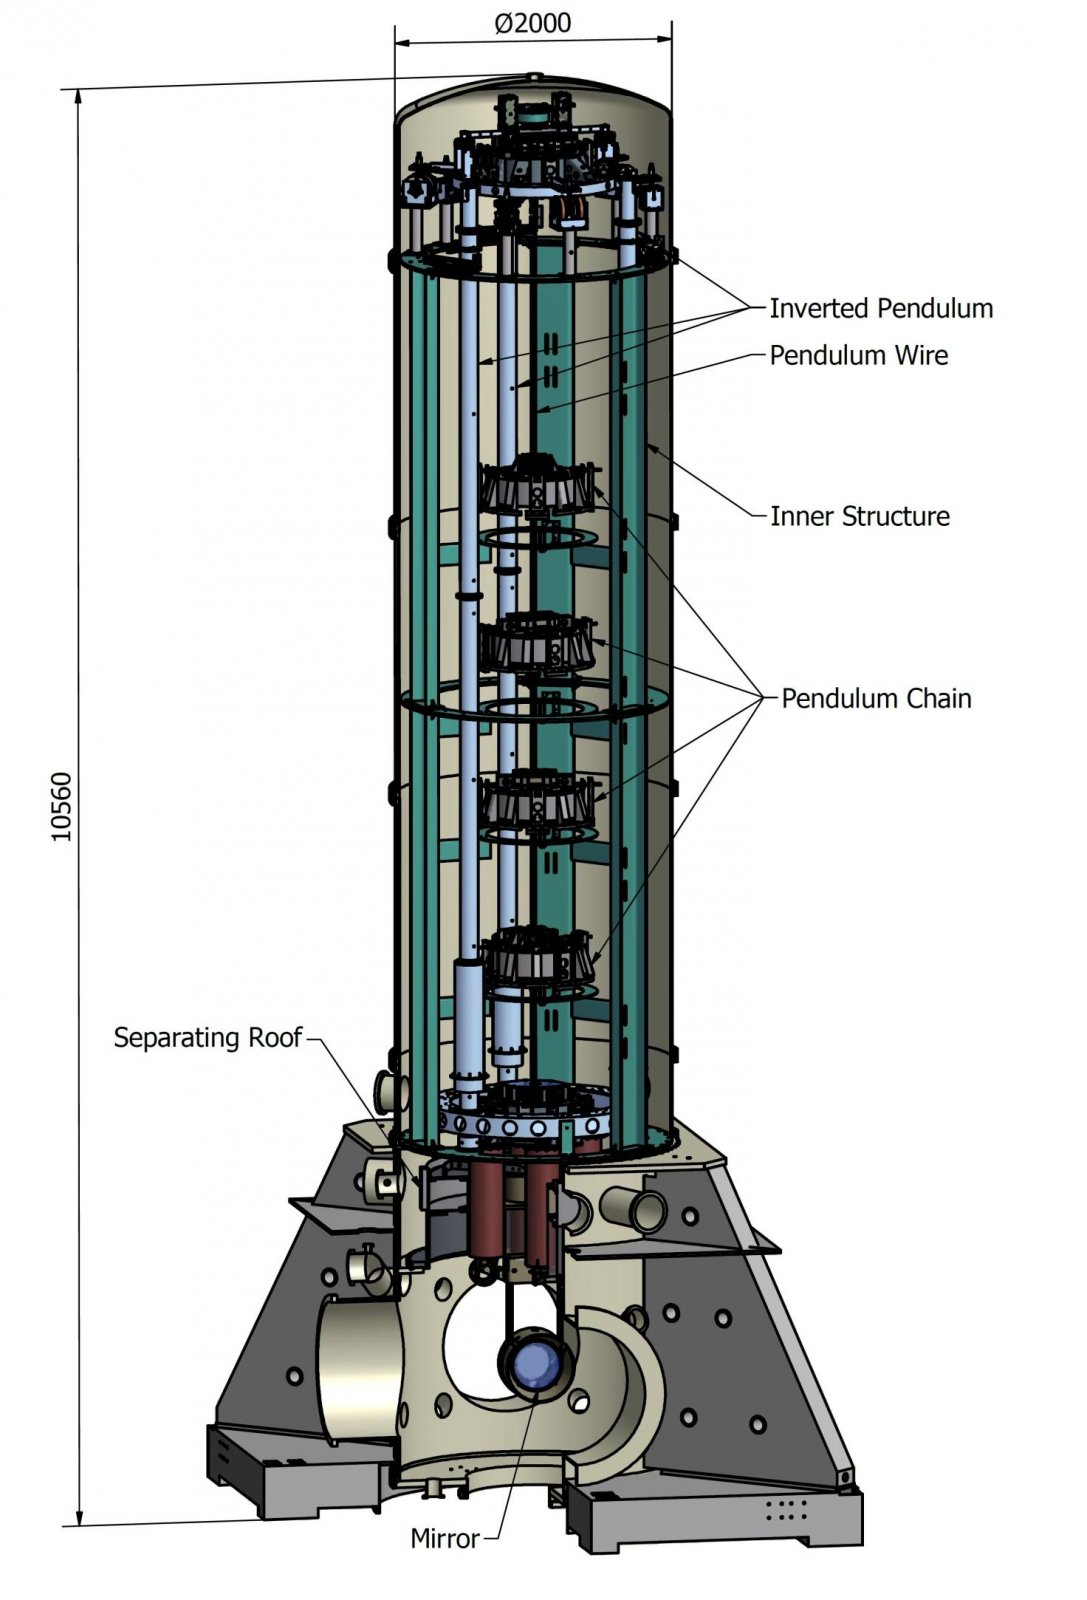
\includegraphics[width=0.5\textwidth]{Figures/superattenuator.jpg}
	\caption{\label{fig:superattenuator}
		A 3D model of the Virgo superattenuator (figure from \cite{Accadia_2012})}
\end{figure}

Similarly to LIGO, Virgo was also equipped with a number of incremental upgrades aimed at improving the sensitivity and testing the maturity of technologies needed for the subsequent version of the detector.
Most notably, the laser power was increased from 10\,W to 25\,W, a thermal compensation system was added, and the test masses were suspended using fused silica fibers directly bonded to the optics to reduce thermal noise\cite{Lorenzini_2010}.
In this configuration, the instrument was referred to as Virgo+.

\subsection{GEO 600 and other detectors}
GEO600~\cite{Grote_2010}, on the other hand, adopted quite different design choices, and pioneered a number of innovative technologies of which several would later be integrated in the larger detectors:
instead of Faby-P\'{e}rot arm cavities it employed folded arms, a topology in which the end of the arms are occupied by folding mirrors that send the laser back towards the end test masses located close to the beam splitter, as shown in the right diagram of \autoref{fig:detector_layouts};
it was the first detector to employ a signal recycling cavity to shape the gravitational wave signal frequency response~\cite{Willke_2002};
it also employed DC readout, rather than the more conventional RF homodyne readout~\cite{DCreadout};
it was the first detector to use monolithic final-stage suspensions of the test-masses~\cite{Plissi_2000};
finally, it was the first to employ squeezing, a technique used to shape quantum fluctuations and obtain a reduction in relative shot noise equivalent to that of a higher power laser~\cite{Grote_2013}.
GEO600 was also the only observatory to remain active during the period in which LIGO and VIRGO were being upgraded to their second generation.

\begin{figure}[htb]
	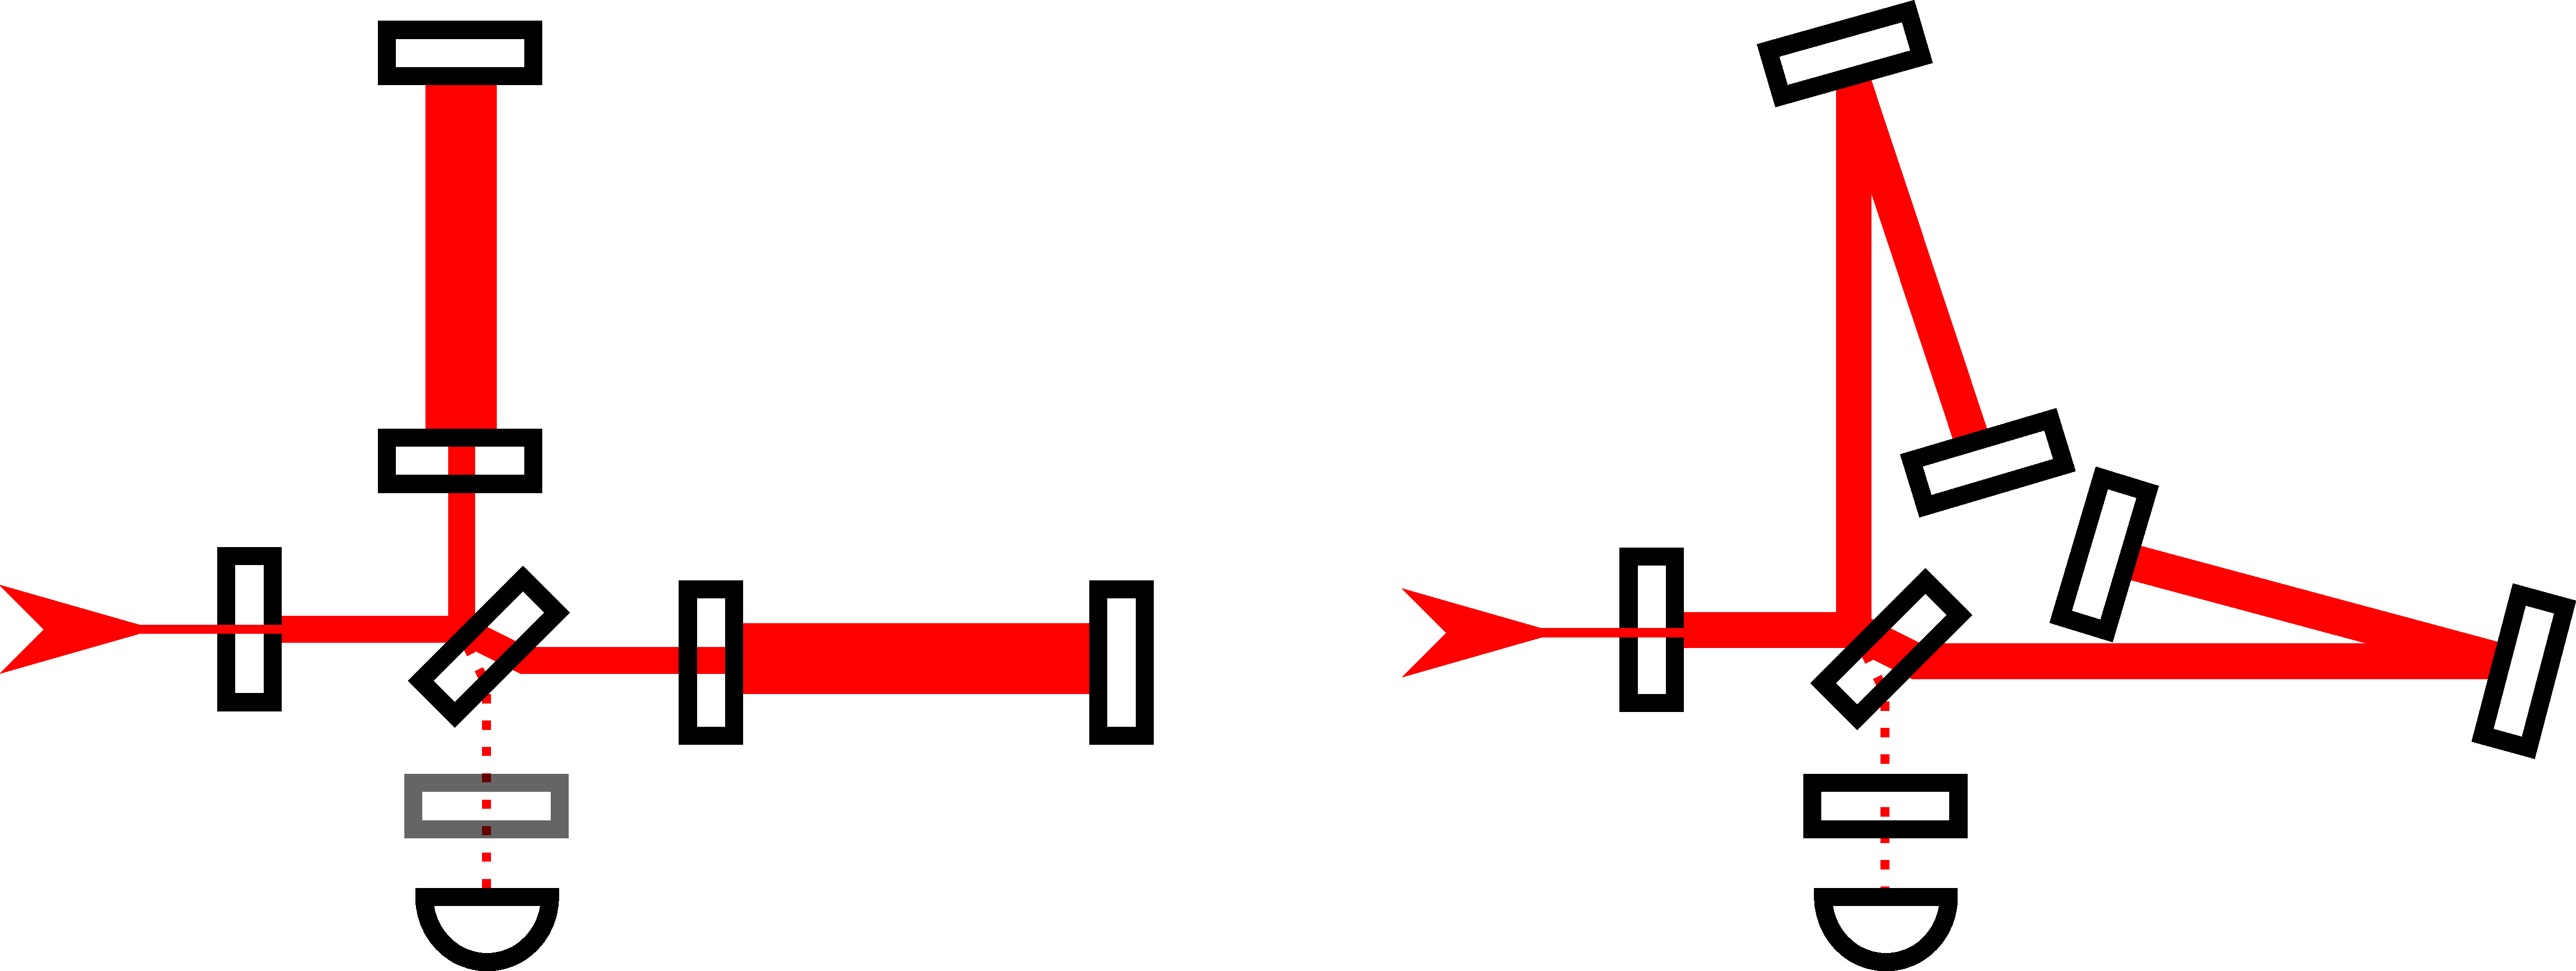
\includegraphics[width=\textwidth]{Figures/detector_layouts.pdf}
	\caption{\label{fig:detector_layouts}
		The optical layouts of the core interferometers of Advanced LIGO and Advanced Virgo (left), and GEO600 (right). 
		In the initial LIGO and Virgo detectors and TAMA300 the optical layout was as shown on the left, bar the omission of the 
signal recycling mirror, shown in the diagram in gray.}
\end{figure}

TAMA300\cite{Ando_2002}, in Japan, also adopted an optical layout similar to LIGO and VIRGO, although its smaller size and location in Tokyo severely limited its sensitivity below a few hundred Hz.
It nevertheless provided many useful results, including the development of sensing and control techniques that would be later transferred to the larger interferometers. 
The CLIO detector, also in Japan but situated in the Kamioka mine, began construction in 2003 and was eventually operated with cryogenically cooled test masses, demonstrating a reduced thermal noise level compared to room temperature~\cite{Uchiyama_2012}. However, with relatively short arm lengths of 100\,m, CLIO could not come close to the strain sensitivities of the larger detectors.

\subsection{Listening for gravitational waves}
In 2002, the LIGO detectors and GEO600 reached a sensitivity adequate for collecting science data, although still far from the design goal.
The first science run took place between August and September 2002 with a conventional range (defined as the maximum distance at which an optimally oriented standard NS-NS coalescence could be detected with a signal-to-noise ratio equal to 8) of 100\,kpc; more than two orders of magnitude less than the design value of 18\,Mpc.
In the years that followed, LIGO conducted other 5 science runs, interrupted by commissioning periods that steadily and consistently improved the performance until it finally reached full design sensitivity in 2006.
In all but one of these observing runs, the three LIGO detectors were run in coincidence with one or more other large scale detectors around the world (GEO600, Virgo and TAMA300) to leverage the superior noise rejection and sky localization capabilities of a widely distributed network of detectors.
In particular Virgo, the only other km-scale detector at the time, reached sufficient sensitivity to participate in an observing run in 2005, and continued joint observation with the LIGO until both were decommissioned in 2010 to start the upgrade process to the advanced detectors \cite{Abbott_2004,Abbott_2005,Abbott_2006,Abbott_2008,Abadie_2010}.
The joint observing runs yielded no detection of gravitational waves, but still produced numerous important scientific outputs, mainly in the form of upper limits (a comprehensive list can be found in \cite{LSCPublications}).

%Approximate list of runs (including partners):
%2002: S1 (LIGO + GEO)
%2003: S2 LIGO + TAMA DT8)
%2004: S3 (LIGO)
%2005: S4 (LIGO + GEO)
%2005-2007: S5 (LIGO + GEO + VIRGO VSR1)
%2009-2010: S6 + VSR2-3 

\subsection{Design and operation of the second generation of interferometric gravitational wave detectors}\label{subsec:2ndgen}

Although no gravitational wave signal had been detected by the first generation of gravitational wave detectors, important scientific outcome had been produced, mostly in the form of upper limits to the amplitude of GW radiation investing the Earth; much more importantly, the scientific community had trained had proved its ability to build and operate such large scale interferometers at their design sensitivity. Time were ripe to move on with the construction of the advanced detectors, designed to have sensitivities sufficient to see at least a few events per year even according to the most pessimistic rate estimates.

In moving to the next generation of detectors, the LIGO and VIRGO projects both followed a similar approach: a complete shutdown of the facilities and replacement of all subsystems with more advanced versions. More powerful lasers, better seismic isolation systems, bigger optics, the introduction of a signal recycling cavity and a more sensitive readout system.

In Japan, the TAMA300 project evolved in LCGT, later renamed KAGRA: a 3-km scale detector to be build in the Kamioka mines near ..., and designed to be operated at cryogenic temperature.
GEO600, despite its limited sensitivity at low frequency, opted to remain the only active detector while the other projects were undergoig construction and upgrades. In the years between 2010 and 2015 it alternated observing runs and commissioning periods, continuing his role of pioneering facility for technologies suitable to be later integrated in the larger interferometers.

%Beside generally aiming at a factor 10 overall improvement in sensitivity, and an expansion fo the sensitive frequency band towards lower frequencies, the design of the advanced detectors was aimed at making them limited by thermal noise, laser radiation pressure and laser shot noise. As a consequence, all other possible sources of noise needed to be pushed well below these main ones.

\subsubsection{Advanced LIGO}

\paragraph*{Suspesions and seismic isolation.}
Two of the subsystems that underwent the biggest upgrades in advanced LIGO as compared to its predecessor were the Seismic Isolation and Suspension subsystems. Although they are formally two separate subsystems, they work in concert to isolate the test-masses and other critical optics from ground vibrations and other macroscopic motions, and ensure that the they can move as free masses in the relevant degree of freedom above a few Hz.

In Advanced LIGO, the test masses are suspended by four-stages pendula. From top to bottom, the main suspension chain is comprised of two metal masses, and two optics of the same shape and size, the lowermost one being the test mass. The first metal mass is attached to the suspension structure by four \textit{spring blades}, which are flexible metal blades providing vertical isolation; steel wires run from the tip of the blades to the suspended mass. In a similar fashion, the second metal mass is attached to the first one, and so is the topmost optic. In the lower stage of the suspension, however, the test mass is attached to the topmost optic by four fused silica fibers; these are directly welded to the two optics in a monolithic assembly, such as to reduce mechanical losses and, consequently, thermal noise. The pendulum resonances of the four stages are distributed between 1 and 4 Hz, providing a passive suppression of motion along the optical axis of $10^-7$ at 10\.Hz, and going down as the frequency to the eighth power.

A similar chain of masses, called reaction chain, hangs parallel to the main one, and supports the sensors and actuators used for local damping and active alignment of the lowermost three masses of the main chain; this provides a quiet reference point for the control forces. The top masses of both chains are instead actuated using the suspension structure as a reference. For all stages except the lowest, the sensors/actuators are compact units that uses shadow sensors to measure the position of, and electromagnets to exert forces on, permanent magnets attached to the masses. The last stage has no local sensors, since the position of the test mass is sensed by the global interferometry; on the end test mass suspensions, the actuators consist of a patterns of electrodes deposited on the last mass of the reaction chain, referred to as reaction mass, which exert electrostatic attractive forces on the test mass when polarized. This avoids the need of attaching magnet or any other part ot the TM, thus maintaining low mechanical losses and reducing possible couplings to external fields. On the input test masses suspension, on the other end, the main laser beam is transmitted through the lowermost optics of both chains; in this case no electrodes are deposited on the reaction mass, that is instead referred to as \textit{compensation plate} for its role in the thermal compensation system, as explained in \ref{sec:presfut:ground:2gen:aLIGO:TCS}.

Each quad suspension is attached to an in-vacuum seismic isolation platforms, used for further suppression of ground vibrations and precise positioning and alignment with a larger range than allowed by the suspensions themselves. The platforms are six-axis, two-stages active and passive isolators proving more than 3 orders of magnitude isolation above 1\.Hz, and positioning capabilities with nm resolution over a range of several mm.

Similar seismic isolation platforms are used to support all the in-vacuum optics; the optics that are part of an optical cavity are installed by triple-pendula, while single-pendulum suspensions, or specialized geometries, are used to isolate less critical optics where necessary.

In both detectors, each of the in-vacuum seismic isolation platforms is installed on beams that are decoupled from the vacuum system itself via flexible bellows, and supported from the outside using hydraulic actuated piers anchored to ground. This systems acts as a further layer of isolation and is used to correct macroscopic positioning correction like the one needed to correct for the moon tidal forces.

%Four 1-m long silica fibers, two per side, connect the test mass to an optic of the same size and shape above it. The fibers are directly welded to both optics in a monolithic assembly to reduce dissipation and consequently thermal noise. The upper optic is then suspended by four steel wires that attach to the tip of as many \textit{blade springs}, flexible metal blades providing vertical isolation. The blade springs are anchored to a metal mass, which is in turn attached to the suspension structure by another four wires and four blade springs.

\paragraph*{Laser}
At freqeuncies above about 100\.Hz, the interferometer sensitivity is limited by shot noise in the laser. The relative impact of the shot noise scales as the inverse of the square root of the power: increasing the laser power is thus a conceptually straightforward way of improving the sensitivity in the shot-noise limited band. The Advanced LIGO laser source is designed to deliver a maximum of 180\.W of laser power, as opposed to the 35\.W used in eLIGO. To obtain this, the eLIGO main laser unit is coupled to an high power laser amplifier (say more about this). The beam is per-stabilized in power, using a reference photodiode, and in frequency, using a thermally controlled refernece optical vacity, before being handed off to the Input Optic subsystem.

\paragraph*{Thermal compensation system}\label{sec:presfut:ground:2gen:aLIGO:TCS}
Despite the stringent requirement on the optical absorption of bulk and coating materials of the optics, the high power levels circulating in the interferometer result in a non-negligible amount of heat released into the optics. Due to the poor heat conduction in vacuum, this induces important thermal gradients that can modify the optical parameters of the system via two main effects: thermal lensing in the bulk material, due to the temperature dependence of the index of refraction, and surface distortion of the high-reflective surfaces, due to thermal expansion. This effect is especially important for the input test masses, since they transmit the most power, and their high-reflective surface is part of the arm cavities of the interferometer.

Initial LIGO already included a thermal compensation system based on CO2 laser that could strategically deliver power to compensate for thermal gradients. This relatively simple system, affected by poor performance and noisy operation, has been radically redesigned for Advanced LIGO. The new thermal compensation system is comprised of two type of actuators: ring heaters, one for each test mass, and CO2 lasers, one for each input test mass. The ring heaters are annular IR emitters that heat the test mass barrel. Their placement is tuned in such a way that the additional thermo-mechanical stress induces a convex deformation of the optic high-reflective surface, thus compensating the central bulge due to the heat released by the laser beam. At the same time, since the laser beam release heat along the axis of the optics, heating from outside reduces the overall thermal gradient and consequently the thermal lensing through the optic.

The ring theater are intended to be tuned to optimally compensate the test mass surface distortion. In general, this results in an only partial compensation fo the thermal lensing. To correct for any residual lensing, the compensation plate is heated by a CO2 laser projector whose pattern can be optimized through the usage of custom masks. The combination of ring heater and CO2 projector on each input thest mass is thus design to fully compensate the geometry of both the reflected and transmitted beams.

The end test masses only have ring heaters, since the transmitted light is used for diagnostic purposes and is not critical to the performance of the instrument.

The thermal compensation system also includes Hartman sensors to monitor the thermal state of the test masses. This kind of sensors works by blocking an incoming beam with a grid of apertures, which result in an array of points being projected on a CCD sensor. The position of each points on the CDD depends on the local curvature of the wavefront of the beam at the corresponding aperture. Any distortion of the wavefront with respect to a reference state is recorded as a relative displacement of the points on the CCD.
In Advanced LIGO, the Hartman sensors use green laser beams injected from the AR face of the test masses, reflected back by the HR face and then directed towards the mask. Each sensor thus monitors the integral effect of a double pass through the substrate thermal lens, and the reflection off the distorted HR surface.

\paragraph*{Optical layout}
The optical layout of Advanced LIGO is different from the initial LIGO layout in several ways. 
Perhaps the most fundamental change to the optical layout is the addition of a signal recycling 
mirror between the anti-symmetric side of the beam splitter and the optical detection port. 
In its current configuration this oft-called signal recycling mirror is actually tuned such as to 
increase the bandwidth of the detector. As such, a more apposite name might be the signal extraction mirror. 

The signal extraction mirror forms a new cavity within Advanced LIGO; the signal recycling cavity. 
Both the signal recycling cavity and the power recycling cavity in Advanced LIGO are designed to be 
geometrically \emph{stable}, by which it should be understood that the round-trip Gouy phase in the cavity 
is significant, and thus higher-order spatial modes are non-degenerate. 
This is contrast to the power recycling cavity in initial LIGO, which was only marginally stable. 
The advantages of the stable recycling cavity design have been clear during the commissioning of 
Advanced LIGO, where commissioning of the length and alignment sensing and control systems has 
been a much smoother process than in initial LIGO. (Tangible advantages of stable recycling cavities). 

Another important geometric change to the optical layout between initial LIGO and Advanced LIGO is 
in the arm cavities. There was a drive towards using larger beam spot sizes on the mirrors in Advanced 
LIGO in order to mitigate the effects of thermal noise. In general there are two cavity geometry solutions available 
that will give a specific beam spot size on the mirrors for a two-mirror cavity of fixed length. The initial LIGO 
arm cavities were designed with a large beam waist inside the cavities, resulting in a cavity g-factor of XXX. 
Advanced LIGO uses the alternative solution of having a small beam waist size in the cavities, giving a cavity g-factor of XXX. 
One of the advantages of the Advanced LIGO arm cavity design is that the relatively large divergence angle of the cavity 
eigenmode reduces the sensitivity of the interferometer to beam tilts (check). 

Several additional optical subsystems have been added in the upgrade from initial LIGO to Advanced LIGO. 
During the enhanced LIGO phase (shortly before initial LIGO went offline for the major upgrade to aLIGO) an output
mode cleaner was added at the output port. The output mode cleaner is a crucial component of the DC readout 
scheme which was first demonstrated in GEO600, and which was determined to be a more optimal solution for 
readout of the gravitational wave signal than the previously used RF heterodyne readout scheme. The output mode 
cleaner subsystem was retained in the aLIGO optical layout, and takes the form of a suspended fixed spacer cavity 
with a bow tie configuration. The output mode cleaner has the essential function of removing RF sidebands and higher-order 
spatial modes from the light incident on the photodiode, this mitigating their impact on the shot noise sensitivity. 

A great effort was made in the upgrade to Advanced LIGO to make the lock acquisition process more deterministic than 
stochastic. Part of this effort was the inclusion of the arm length stabilization (ALS) subsystem. This subsystem consists uses 
green frequency-doubled Nd:YAG beams which are phased locked to the main laser to independently control the arm cavities during 
lock acqusition of the central dual-recycled Michelson interferometer (DRMI). Once the DRMI is locked the ALS can be used 
methodically bring the arms to resonance, bringing the full interferometer to the ideal operating point.

\paragraph*{Interferometric sensing and control}
The dual-recycled Fabry-Perot Michelson interferometer that makes up aLIGO has a very narrow linear range. 
The practical consequence of this fact, combined with the fact that with only passive seismic isolation systems typical 
mirror motions at low frequencies can be of the order several wavelengths, is that length control loops are essential in order 
to keep the interferometer within the linear range. 

The length sensing of aLIGO is based on the Pound-Drever-Hall laser frequency stabilization scheme~\ref{PDH}. 
This scheme is based on adding RF phase modulation sidebands to the carrier light, which are well outside the linewidth 
of the optical cavity 
to be used as the frequency reference. When the carrier light frequency is brought within one linewidth of the cavity, 
the carrier picks up a phase shift in reflection of the cavity which is proportional to the difference between carrier light 
frequency and the cavity resonant frequency. The sidebands can then act as a phase reference, because being far outside 
the cavity linewidth. ji


\begin{itemize}
\item length sensing and control, PDH
\item sideband frequencies, resonances in certain cavities
\item Schnupp asymmetry
\item DC offset
\item ESDs
\item ASC
\end{itemize}

signal recycling. I actually think this should maybe just go under optical layout.
Maybe also have a section for noise budget, or sensitivity curve?








Aside from the addition of the signal recycling mirror, the most notable change from the initial LIGO optical 
layout is the stable design of the recycling cavities.


\subsubsection{Advanced Virgo}
\begin{itemize}
\item Sesmic isolation upgrade?
\item Laser power upgrade
\item Optical layout
\item sensing and control
\item Thermal compensation
\item signal recyling
\end{itemize}

 

\subsection{The future of ground based interferometric gravitational wave detection}\label{subsec:future}

After the announcement of the first detection of gravitational waves by the LIGO-Virgo collaboration, the anticipation for an extended network of detectors to come online became even more pressing.
Now that the possibility of detecting gravitational waves had been proven, the scientific community was looking forward to the science that can be done by collecting and analyzing a large number of events with well constrained parameters.
A network of three or more detectors would improve on a number of key factors, including the coincident duty cycle, better parameter estimation and much more precise sky localization. The latter is fundamental to increase the odd of simultaneously observing an event in both the GW and EM spectra, thus enabling the so called \textit{multi-messenger astronomy}.

Virgo was already expected to join the second LIGO observing run starting in summer 2016, and despite some installation and commissioning issues, the LIGO and Virgo communities are working hard to make it happen.

It was not originally planned for Kagra to join the network with meaningful sensitivity before 2018, and various delays are pushing the schedule back even more. 
The managing team went trough a redefinition of the schedule in winter 2016, and outlined a plan to skip an intermediate commissioning phase and accelerate the path to the final, cryogenic version of the detector. 
In spring 2016 the interferometer was locked for the first time in a simple Michelson configuration with no arm cavities or recycling cavities, but using the full 3\,km arm-length.

The announcement of the detection of GW150914 also gave a decisive impulse to the LIGO India project.
As for Initial LIGO, the Advanced LIGO project included two interferometers to be installed in the Hanford site vacuum system.
Unlike for Initial LIGO, the second interferometer was designed to be 4\,km long, rather than 2\,km. 
Shortly after the installation phase began, an idea started to take hold in the community: what if, instead of building two co-located interferometers that would be affected by the same disturbances and not add much to the science output, the third instrument could be moved to a completely different location? 
If a country was willing to invest in the construction of the infrastructure and vacuum system, it would be rewarded with the ability to jump to the forefront of gravitational wave science by borrowing from the Advanced LIGO project all the instrumentation that was designed and built for the second Hanford detector. 
Besides likely improving the overall network duty cycle, a strategic placement of the additional detector would also greatly improve the parameter estimation and localization capability of the network~\cite{Klimenko_2016}.
Australia was initially identified as a possible partner; when funding constraints made it clear that the deal could not happen on fruitful time scales, India stepped in.
The project seemed to move quickly at the beginning, with the INDIGO (the Indian gravitational wave community) management putting forward a great effort to train their scientists, complete site surveys and make all other necessary preparations, with great help and support by the LIGO management. 
Unfortunately, a change in government slowed process almost to a halt in 2015. 
It was only after the announcement of the first discovery by the LIGO project that the Indian government approved the project. 
Although the detector is not projected to come online before 2022, this represents an important success that will strategically expand the network of GW detectors and the list of countries involved.

In the meanwhile, the LIGO project is already researching possible upgrades, to be developed and installed in a few years time-frame in the current detectors without the need of a complete rebuild.
Such upgrades includes frequency dependent squeezing, heavier test masses, improved coating, suspensions with reduced thermal noise and strategies to subtract Newtonian noise.
Proposals are also being considered to cool down the test masses, thus reducing thermal noise in coating and suspensions. 
%Plans are also underway to begin a design study for a next generation LIGO facility, tentatively titled \emph{LIGO cosmic explorer}, that may include longer beam tubes capable of housing a detector with a sensitivity 10 times that of Advanced LIGO across the detection band~\cite{Dwyer2015}. 

Despite the factor of few improvement in overall sensitivity attainable with the above mentioned upgrades, the GW community is starting to realize that a substantial gains in maximum and low-frequency sensitivity will require to abandon the current infrastructures. 
Different studies are being carried out to shape the concept of the next generation of ground detector, including a proposal in the LIGO community to move to a detector of essentially the same design, but substantially increased length~\cite{Dwyer2015}.
The most advanced and well studied concept, however, has been developed by the European community for a detector dubbed Einstein Telescope~\cite{Punturo2010}.
The observatory would be built about 150\,m underground, in a system of galleries forming a 10\,km side horizontal equilateral triangle. Three detectors would be co-located in the facility, with each vertex of the triangle hosting the corner station of one, and the end stations of other two.
Each detector would actually be comprised of two dual-recycled, Fabry-P\'{e}rot Michelson  interferometers, sharing the same geometrical arrangement but optimized for two different frequencies bands: a cryogenic, low power one for the lower frequency sensitivity, and a room temperature more powerful version for higher frequency sensitivity.

Compared to any one of the current observatories, the six interferometers combined would exhibit a much more uniform antenna pattern, in terms of both sky-position and polarization of the sources, improve the maximum sensitivity by more than a factor of 10 and allow to observe signals down to about 1\,Hz. 
Their proposed design is based on technologies that are currently state of the art, or have a mature enough state of development to make solid prediction about their future performance possible; however, the ET community has made clear that one of the main goal of the proposal is that of building an infrastructure for an observatory expected to remain current for decades, while the hosted instrumentation is upgraded according to the latest developments.

The nature of the field of gravitational wave detection is such that it may be many years before a new breakthrough technology with the power to improve the strain sensitivity makes it from the conceptual stage to real implementation in a full scale detector. 
As such, research groups around the world are already working hard on developing the technologies of the future, perhaps a decade or more before they might make it into the vacuum enclosures and clean rooms of the future instruments. 
This constant drive for better sensitivity makes the field a very creative one, and one in which there can be expected to be many years of innovation and technical achievements still to come, even after the first direct detection of gravitational waves. 

%TODO: need a proof-read of the final bibliography (as printed). Should wait for answer about author formatting to come from editors.
\bibliographystyle{ws-rv-van}    % Bibliography: Author-Date system
\bibliography{presentandfuture}      % pls. call your database here